\documentclass[../thesis.tex]{subfiles}

\begin{document}
    \section{Snell's Law}
    \label{sec:snells-law}

    The law of refraction by \textsc{Snell} describes relation between the angles of incidence and refraction of an electromagnetic wave that passes from a medium with refractive index $n_1$ to a medium with the index $n_2$. It is derived from \textsc{Fermat}'s principle, which implies that an electromagnetic wave traveling from point $A$ to point $B$ always takes the fastest path possible. Using the dependency of the speed of light on the index of refraction of a medium
    \begin{equation}
        v_i = \frac{c}{n_i},
    \end{equation}
    according to figure \cref{fig:snells-law}, the wave takes the time
    \begin{equation}
        t=\frac{\sqrt{x^2 + a^2}}{v_1} + \frac{\sqrt{(l-x)^2 + b^2}}{v_2}
        \label{eq:snell}
    \end{equation}
    to travel from $A$ to $C$. To find the shortest possible time depending on the parameter $x$, equation \cref{eq:snell} is derived and equated to zero yielding the \textsc{Snell}'s law
    \begin{equation}
        n_1 \sin\left(\alpha\right) = n_2 \sin\left(\beta\right).
        \label{eq:snells-law}
    \end{equation}

    \subfile{tikz/optics/snells_law.tex}


    \section{Fresnel Equations}
    \label{sec:fresnel-equations}

        The \textsc{Fresnel} equations describe the transmission and reflection coefficients of an electromagnetic wave passing from a medium with a refractive index $n_1$ to a medium with refractive index $n_2$. They are derived from the \textsc{Maxwell} equations and the \textsc{Snell}'s law as follows. An electromagnetic wave hitting an interface as described above is partially reflected and partially transmitted. The law of reflection yields the reflection angle
        \begin{equation}
            \theta_\mathrm{r} = \theta_\mathrm{i},
        \end{equation}
        where $\theta_\mathrm{i}$ is the incident angle (compare figure \cref{fig:fresnel-equations}). Moreover, the transmitted part behaves according to \textsc{Snell}'s law resulting in the angle $\theta_\mathrm{t}$ (section \cref{sec:snells-law}). In the following, only o-polarized waves shall be regarded. The \textsc{Maxwell} equations yield the electromagnetic boundary conditions
        \begin{equation}
            \begin{split}
                E_\mathrm{i}\cos\theta_\mathrm{i} + E_\mathrm{r}\cos\theta\mathrm{i} &= E_\mathrm{t}\cos\theta\mathrm{t}    \\
                H_\mathrm{i} - H_\mathrm{r} &= H_\mathrm{t}.
                \label{eq:boundary-cond-1}
            \end{split}
        \end{equation}
        In words, the components of the magnetic field $H_\parallel$ and the electric field $E_\parallel$ are continuous. Using
        \begin{align}
            \begin{split}
                H&=\sqrt{\frac{\epsilon}{\mu}}E \\
                n&=c\sqrt{\epsilon\mu}
            \end{split}
            \label{eq:boundary-cond-2}
        \end{align}
        to solve the equations \cref{eq:boundary-cond-1} yields the \textsc{Fresnel} equations
        \begin{align}
            \begin{split}
                r_\mathrm{p} &= \frac{E_\mathrm{r}^\mathrm{p}}{E_\mathrm{i}^\mathrm{p}} = \frac{\frac{n_1}{\mu_1}\cos\theta_\mathrm{t} - \frac{n_2}{\mu_2}\cos\theta_\mathrm{i}}{\frac{n_1}{\mu_1}\cos\theta_\mathrm{t} + \frac{n_2}{\mu_2}\cos\theta_\mathrm{i}} \\
                t_\mathrm{p} &= \frac{E_\mathrm{t}^\mathrm{p}}{E_\mathrm{i}^\mathrm{p}} = \frac{2\frac{n_1}{\mu_1}\cos\theta_\mathrm{t}}{\frac{n_1}{\mu_1}\cos\theta_\mathrm{t} + \frac{n_2}{\mu_2}\cos\theta_\mathrm{i}}.
            \end{split}
            \label{eq:fresnel1}
        \end{align}
        Assuming non magnetic materials, in explanation
        \begin{equation}
            \mu_1 = \mu_2 ) \mu_0,
        \end{equation}
        and using \textsc{Snell}'s law to simplify, \cref{eq:fresnel1} becomes
        \begin{align}
            \begin{split}
                r_\mathrm{p} &= \frac{n_1\cos\theta_\mathrm{t}-n_2\cos\theta_\mathrm{t}}{n_1\cos\theta_\mathrm{t}+n_2\cos\theta_\mathrm{t}}  \\
                t_\mathrm{p} &= \frac{2n_1\cos\theta_\mathrm{i}}{n_1\cos\theta_\mathrm{t}+n_2\cos\theta_\mathrm{t}}.
            \end{split}
            \label{eq:fresnel2}
        \end{align}

        \subfile{tikz/optics/fresnel_equations.tex}


        \subsection{Two Interface Transmission}
        \label{subsec:two_interface_trans}

            \subfile{tikz/optics/transmission_two_layers.tex}

            In this section, the transmission of an electromagnetic wave through two media of increasing refractive indices
            \begin{equation}
                1 = n_1 < n_2 < n_3
                \label{eq:nstep}
            \end{equation}
            shall be compared to that a single interface transmission with
            \begin{equation}
                1 = n_1 < n_3.
            \end{equation}
            Figure \cref{fig:two-layer-transmission} shows the two situations and defines the respective angles. To simplify the situation further
            \begin{equation}
                \alpha = 0
                \label{eq:alpha0}
            \end{equation}
            shall be assumed as the incident angle. Hereby, the \textsc{Fresnel} transmission coefficient \cref{eq:fresnel2} becomes
            \begin{equation}
                t_\mathrm{p} = \frac{2n_1}{n_1+n_2}
            \end{equation}
            as by \textsc{Snell}'s law \cref{eq:alpha0} makes for
            \begin{equation}
                \alpha = \beta =\gamma = \delta = 0.
            \end{equation}
            Because more diffracting matter is added to the system, the two interface transmission is expected to yield a lower transmission than the single interface transmission, even though refractive index contrasts
            \begin{equation}
                \Delta n = n_i - n_j, \quad \{i,j\}\in\{1,2,3\},
            \end{equation}
            are smaller. Therefore, the inequality
            \begin{align}
                \begin{split}
                    t_\mathrm{p}^{13} &> t_\mathrm{p}^{123} = t_\mathrm{p}^{12} \cdot t_\mathrm{p}^{23}\\
                    \frac{2n_1}{n_1+n_3} &> \frac{2n1}{n_1+n_2}\cdot\frac{n_2}{n_2+n_3}
                \end{split}
                \label{eq:inequality}
            \end{align}
            is regarded. With figure \cref{fig:inequality-solution} \cref{eq:inequality} is solved graphically. The yielded result is that the transmission of the two interface transmission is indeed weaker than for the single interface assuming the inequality \cref{eq:nstep}.

            \begin{figure}[ht]
                \centering
                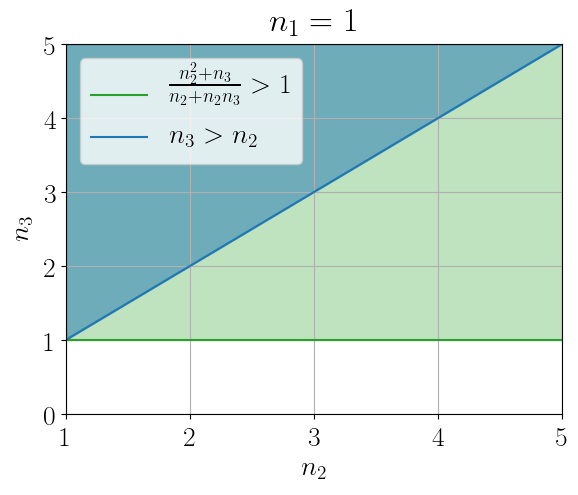
\includegraphics[width=0.6\textwidth]{images/inequality.png}
                \caption{Graphical solution of the inequality \cref{eq:inequality}. While the blue shaded area also respects the inequality \cref{eq:nstep}, the orange shaded area shows the more general case $1=n_1<n_2,n_3$. Both cases yield a weaker transmission for the two interface transmission than for the single interface.}
                \label{fig:inequality-solution}
            \end{figure}


    \section{Blablabla Näherung}
    \label{sec:porous-transmission}

        The refractive index of a porous medium with structures in the range of the wavelength of the transmitting light can be approximated by the blablabla???. Using the porosity $0<\phi<1$ as a parameter it is assumed that the effective refractive index behaves like
        \begin{equation}
            n_\mathrm{eff} = n_1 \left(1-\phi\right) + n_2 \phi
            \label{eq:porous-transmission-approximation}
        \end{equation}
        where $n_{1,2}$ are the indices of the two components the medium is composed off (for nanoporous alumina membranes in empty state the components are alumina and vacuum for example).

        \subfile{tikz/optics/porous_n.tex}


        \subsection{Transmission of Nanoporous Membranes in Empty and Filled State}

            Here, nanoporous media made of an arbitrary material with the sole condition that $n_\mathrm{mat}>1$ shall be regarded in empty and filled state. The wetting liquid's refractive index be $n_\mathrm{liq}>1$. The approximation \cref{eq:porous-transmission-approximation} yields the inequality
            \begin{equation}
                n_\mathrm{eff}^\mathrm{empty}=n_1\cdot\left( 1-\phi\right) + n_\mathrm{vac}\cdot\phi <n_1 \left( 1-\phi\right) +n_\mathrm{liq}\phi =n_\mathrm{eff}^\mathrm{filled},
                \label{eq:neff-inequality}
            \end{equation}
            where
            \begin{equation}
                1=n_\mathrm{vac}<n_\mathrm{liq}
            \end{equation}
            with the refractive index of vacuum $n_\mathrm{vac}$. Referring to \cref{eq:fresnel2} yields the transmission coefficients
            \begin{equation}
                T_\mathrm{empty}=\left(\frac{2n_\mathrm{vac}}{n_\mathrm{vac}+n_\mathrm{eff}^\mathrm{empty}}\right)^2 \stackrel{\text{\cref{eq:neff-inequality}}}{>} \left(\frac{2n_\mathrm{vac}}{n_\mathrm{vac}+n_\mathrm{eff}^\mathrm{filled}}\right)^2=T_\mathrm{filled}
            \end{equation}
            when assuming an incident angle $\theta_\mathrm{i}=0$ once again.


            \subsubsection{Transmission of Empty AAM Membrane}

                To give an example, the transmission coefficient of an empty nanoporous alumina membrane as used in the conducted experiments is computed in the following. The alumina membranes parameters are
                \begin{align}
                    \phi &= \SI{25}{\percent}   \\
                    n_{\ce{Al2O3}} &= 1,7682   %https://refractiveindex.info/?shelf=main&book=Al2O3&page=Malitson-o
                \end{align}
                which make for a transmission coefficient of
                \begin{equation}
                    T_{\ce{Al2O3}}^\mathrm{empty}=0,9024.
                \end{equation}


    \section{Rayleigh Scattering}
    \label{sec:rayleigh-scattering}


        \section{Index Matching}
        \label{sec:index-matching}


\end{document}
